\chapter{Strings and things}
\label{strings}

\index{object}
\index{System.in}
\index{System.out}

In Java and other object-oriented languages, an {\bf object} is a collection of data that provides a set of methods.
For example, \java{Scanner}, which we saw in Section~\ref{scanner}, is an object that provides methods for parsing input.
\java{System.out} and \java{System.in} are also objects.

Strings are objects, too.
They contain characters and provide methods for manipulating character data.
We explore some of those methods in this chapter.

\index{primitive}

Not everything in Java is an object: \java{int}, \java{double}, and \java{boolean} are so-called {\bf primitive} types.
We will explain some of the differences between object types and primitive types as we go along.


\section{Characters}

\index{charAt}
\index{char}
\index{type!char}

Strings provide a method named \java{charAt}, which extracts a character.
It returns a \java{char}, a primitive type that stores an individual character (as opposed to strings of them).

\begin{code}
String fruit = "banana";
char letter = fruit.charAt(0);
\end{code}

The argument \java{0} means that we want the letter at position 0.
Like array indexes, string indexes start at 0, so the character assigned to \java{letter} is \java{b}.

Characters work like the other primitive types we have seen.
You can compare them using relational operators:

\begin{code}
if (letter == 'a') {
    System.out.println('?');
}
\end{code}

\index{quote mark}
\index{escape sequence}

Character literals, like \java{'a'}, appear in single quotes.
Unlike string literals, which appear in double quotes, character literals can only contain a single character.
Escape sequences, like \java{'\\t'}, are legal because they represent a single character.

The increment and decrement operators work with characters.
So this loop displays the letters of the alphabet:

\begin{code}
System.out.print("Roman alphabet: ");
for (char c = 'A'; c <= 'Z'; c++) {
    System.out.print(c);
}
System.out.println();
\end{code}

\index{Unicode}

Java uses {\bf Unicode} to represent characters, so strings can store text in other alphabets like Cyrillic and Greek, and non-alphabetic languages like Chinese.
You can read more about it at \url{http://unicode.org/}.

In Unicode, each character is represented by a ``code point'', which you can think of as an integer.
The code points for uppercase Greek letters run from 913 to 937, so we can display the Greek alphabet like this:

\begin{code}
System.out.print("Greek alphabet: ");
for (int i = 913; i <= 937; i++) {
    System.out.print((char) i);
}
System.out.println();
\end{code}

This example uses a type cast to convert each integer (in the range) to the corresponding character.


\section{Strings are immutable}
\label{immutable}

\index{toUpperCase}
\index{toLowerCase}
\index{immutable}

Strings provide methods, \java{toUpperCase} and \java{toLowerCase}, that convert from uppercase to lowercase and back.
These methods are often a source of confusion, because it sounds like they modify strings.
But neither these methods nor any others can change a string, because strings are {\bf immutable}.

When you invoke \java{toUpperCase} on a string, you get a new string object as a return value.
For example:

\begin{code}
String name = "Alan Turing";
String upperName = name.toUpperCase();
\end{code}

\index{Turing, Alan}

After these statements run, \java{upperName} refers to the string \java{"ALAN TURING"}.
But \java{name} still refers to \java{"Alan Turing"}.

\index{replace}

Another useful method is \java{replace}, which finds and replaces instances of one string within another.
This example replaces \java{"Computer Science"} with \java{"CS"}:

\begin{code}
String text = "Computer Science is fun!";
text = text.replace("Computer Science", "CS");
\end{code}

This example demonstrates a common way to work with string methods.
It invokes \java{text.replace}, which returns a reference to a new string, \java{"CS is fun!"}.
Then it assigns the new string to \java{text}, replacing the old string.

This assignment is important; if you don't save the return value, invoking \java{text.replace} has no effect.

% ABD: Too many new ideas here: the most important one is that you have to do something with the return value.  It's not a good time to appreciate the glory of immutability.

%Strings are immutable by design, because it simplifies passing them between methods as parameters and return values.
%And since the contents of a string can never change, two variables can reference the same string without one accidentally corrupting the other.


\section{String traversal}
\label{stringtraverse}

\index{traverse}

The following loop traverses the characters in \java{fruit} and displays them, one on each line:

\begin{code}
for (int i = 0; i < fruit.length(); i++) {
    char letter = fruit.charAt(i);
    System.out.println(letter);
}
\end{code}

\index{string!length}
\index{length!string}

Strings provide a method called \java{length} that returns the number of characters in the string.
Because it is a method, you have to invoke it with the empty argument list, \java{()}.
%Do not confuse \java{string.length()}, which is a method, with \java{array.length}, which is a constant.

\index{loop variable}
\index{variable!loop}

The condition is \java{i < fruit.length()}, which means that when \java{i} is equal to the length of the string, the condition is \java{false} and the loop terminates.

\index{toCharArray}

Unfortunately, the enhanced \java{for} loop does not work with strings.
But you can convert any string to a character array and iterate that:

\begin{code}
for (char letter : fruit.toCharArray()) {
    System.out.println(letter);
}
\end{code}

To find the last letter of a string, you might be tempted to try something like:

\begin{code}
int length = fruit.length();
char last = fruit.charAt(length);      // wrong!
\end{code}

\index{StringIndexOutOfBoundsException}
\index{exception!StringIndexOutOfBounds}

This code compiles and runs, but invoking the \java{charAt} method throws a \java{StringIndexOutOfBoundsException}.
The problem is that there is no sixth letter in \java{"banana"}.
Since we started counting at 0, the 6 letters are indexed from 0 to 5.
To get the last character, you have to subtract 1 from \java{length}.

\begin{code}
int length = fruit.length();
char last = fruit.charAt(length - 1);  // correct
\end{code}

Many string traversals involve reading one string and creating another.
For example, to reverse a string, we simply add one character at a time:

\begin{code}
public static String reverse(String s) {
    String r = "";
    for (int i = s.length() - 1; i >= 0; i--) {
        r = r + s.charAt(i);
    }
    return r;
}
\end{code}

\index{empty string}

The initial value of \java{r} is \java{""}, which is the {\bf empty string}.
The loop traverses the letters of \java{s} in reverse order.
Each time through the loop, it creates a new string and assigns it to \java{r}.
When the loop exits, \java{r} contains the letters from \java{s} in reverse order.
So the result of \java{reverse("banana")} is \java{"ananab"}.


\section{Substrings}

The \java{substring} method returns a new string that copies letters from an existing string, starting at the given index.

\begin{itemize}
\item \java{fruit.substring(0)} returns \java{"banana"}
\item \java{fruit.substring(2)} returns \java{"nana"}
\item \java{fruit.substring(6)} returns \java{""}
\end{itemize}

The first example returns a copy of the entire string.
The second example returns all but the first two characters.
As the last example shows, \java{substring} returns the empty string if the argument is the length of the string.

To visualize how the \java{substring} method works, it helps to draw a picture like Figure~\ref{fig.banana}.

\begin{figure}[!ht]
\begin{center}
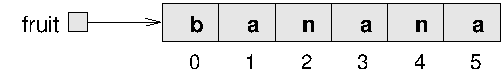
\includegraphics{figs/banana.pdf}
\caption{Memory diagram for a \java{String} of six characters.}
\label{fig.banana}
\end{center}
\end{figure}

%\begin{center}
%\begin{tabular}{c|c|c|c|c|c}
%%\hline
%b & a & n & a & n & a \\
%\hline
%0 & 1 & 2 & 3 & 4 & 5 \\
%%\hline
%\end{tabular}
%\end{center}

Like most string methods, \java{substring} is overloaded.
That is, there are other versions of \java{substring} that have different parameters.
If it's invoked with two arguments, they are treated as a start and end index:

\begin{itemize}
\item \java{fruit.substring(0, 3)} returns \java{"ban"}
\item \java{fruit.substring(2, 5)} returns \java{"nan"}
\item \java{fruit.substring(6, 6)} returns \java{""}
\end{itemize}

Notice that the character indicated by the end index is not included.
Defining \java{substring} this way simplifies some common operations.
For example, to select a substring with length \java{len}, starting at index \java{i}, you could write \java{fruit.substring(i, i + len)}.


\section{The indexOf method}

\index{indexOf}

The \java{indexOf} method searches for a character in a string.

\begin{code}
String fruit = "banana";
int index = fruit.indexOf('a');
\end{code}

This example finds the index of \java{'a'} in the string.
But the letter appears three times, so it's not obvious what \java{indexOf} should do.
According to the documentation, it returns the index of the {\em first} appearance.

To find subsequent appearances, you can use another version of \java{indexOf}, which takes a second argument that indicates where in the string to start looking.

\begin{code}
int index = fruit.indexOf('a', 2);
\end{code}

This code starts at index 2 (the first \java{'n'}) and finds the next \java{'a'}, which is at index 3.
If the letter happens to appear at the starting index, the starting index is the answer.
So \java{fruit.indexOf('a', 5)} returns \java{5}.

If the character does not appear in the string, \java{indexOf} returns \java{-1}.
Since indexes cannot be negative, this value indicates the character was not found.

You can also use \java{indexOf} to search for a substring, not just a single character.
For example, the expression \java{fruit.indexOf("nan")} returns \java{2}.


\section{String comparison}
\label{strcmp}

\index{equals}
\index{compareTo}

To compare two strings, it may be tempting to use the \java{==} and \java{!=} operators.

\begin{code}
String name1 = "Alan Turing";
String name2 = "Ada Lovelace";
if (name1 == name2) {                 // wrong!
    System.out.println("The names are the same.");
}
\end{code}

This code compiles and runs, and most of the time it gets the answer right.
But it is not correct, and sometimes it gets the answer wrong.
The problem is that the \java{==} operator checks whether the two variables refer to the same object (by comparing the references).
If you give it two different strings that contain the same letters, it yields \java{false}.

The right way to compare strings is with the \java{equals} method, like this:

\begin{code}
if (name1.equals(name2)) {
    System.out.println("The names are the same.");
}
\end{code}

This example invokes \java{equals} on \java{name1} and passes \java{name2} as an argument.
The \java{equals} method returns \java{true} if the strings contain the same characters; otherwise it returns \java{false}.

If the strings differ, we can use \java{compareTo} to see which comes first in alphabetical order:

\begin{code}
int diff = name1.compareTo(name2);
if (diff == 0) {
    System.out.println("The names are the same.");
} else if (diff < 0) {
    System.out.println("name1 comes before name2.");
} else if (diff > 0) {
    System.out.println("name2 comes before name1.");
}
\end{code}

The return value from \java{compareTo} is the difference between the first characters in the strings that differ.
If the strings are equal, their difference is zero.
If the first string (the one on which the method is invoked) comes first in the alphabet, the difference is negative.
Otherwise, the difference is positive.

In the preceding code, \java{compareTo} returns positive 8, because the second letter of \java{"Ada"} comes before the second letter of \java{"Alan"} by 8 letters.

\index{case-sensitive}

Both \java{equals} and \java{compareTo} are case-sensitive.
The uppercase letters come before the lowercase letters, so \java{"Ada"} comes before \java{"ada"}.


\section{String formatting}

\index{printf}
\index{utility method}

In Section~\ref{printf}, we learned how to use \java{printf} to display formatted output.
Sometimes programs need to create strings that are formatted a certain way, but not display them immediately, or ever.
For example, the following method returns a time string in 12-hour format:

\begin{code}
public static String timeString(int hour, int minute) {
    String ampm;
    if (hour < 12) {
        ampm = "AM";
        if (hour == 0) {
            hour = 12;  // midnight
        }
    } else {
        ampm = "PM";
        hour = hour - 12;
    }
    return String.format("%02d:%02d %s", hour, minute, ampm);
}
\end{code}

\index{string!format}

\java{String.format} takes the same arguments as \java{System.out.printf}: a format specifier followed by a sequence of values.
The main difference is that \java{System.out.printf} displays the result on the screen; \java{String.format} creates a new string, but does not display anything.

In this example, the format specifier \java{\%02d} means ``two digit integer padded with zeros'', so \java{timeString(19, 5)} returns the string \java{"07:05 PM"}.


\section{Wrapper classes}
\label{wrappers}

Primitive values (like \java{int}s, \java{double}s, and \java{char}s) do not provide methods.
For example, you can't call \java{equals} on an \java{int}:

\begin{code}
int i = 5;
System.out.println(i.equals(5));  // compiler error
\end{code}

\index{wrapper class}
\index{Character}
\index{Integer}
\index{Double}

But for each primitive type, there is a corresponding class in the Java library, called a {\bf wrapper class}.
The wrapper class for \java{char} is called \java{Character}; for \java{int} it's called \java{Integer}.
Other wrapper classes include \java{Boolean}, \java{Long}, and \java{Double}.
They are in the \java{java.lang} package, so you can use them without importing them.

Each wrapper class defines constants \java{MIN_VALUE} and \java{MAX_VALUE}.
For example, \java{Integer.MIN_VALUE} is \java{-2147483648}, and \java{Integer.MAX_VALUE} is \java{2147483647}.
Because these constants are available in wrapper classes, you don't have to remember them, and you don't have to include them in your programs.

Wrapper classes provide methods for converting strings to other types.
For example, \java{Integer.parseInt} converts a string to (you guessed it) an integer:

\begin{code}
String str = "12345";
int num = Integer.parseInt(str);
\end{code}

\index{parse}

In this context, {\bf parse} means something like ``read and translate''.

The other wrapper classes provide similar methods, like \java{Double.parseDouble} and \java{Boolean.parseBoolean}.
They also provide \java{toString}, which returns a string representation of a value:

\begin{code}
int num = 12345;
String str = Integer.toString(num);
\end{code}

The result is the string \java{"12345"}.


\section{Command-line arguments}

Now that you know about arrays and strings, we can {\em finally} explain the \java{args} parameter for \java{main} that we have been ignoring since Chapter~\ref{theway}.
If you are unfamiliar with the command-line interface, please read or review Appendix~\ref{commandline}.

Continuing an earlier example, let's write a program to find the largest value in a sequence of numbers.
Rather than read the numbers from \java{System.in}, we'll pass them as command-line arguments.
Here is a starting point:

\begin{code}
public class Max {
    public static void main(String[] args) {
        System.out.println(Arrays.toString(args));
    }
}
\end{code}

You can run this program from the command line by typing:

\begin{stdout}
java Max
\end{stdout}

\index{empty array}

The output indicates that \java{args} is an {\bf empty array}; that is, it has no elements:

\begin{stdout}
[]
\end{stdout}

But if you provide additional values on the command line, they are passed as arguments to \java{main}.
For example, if you run it like this:

\begin{stdout}
java Max 10 -3 55 0 14
\end{stdout}

The output is:

\begin{stdout}
[10, -3, 55, 0, 14]
\end{stdout}

But remember that the elements of \java{args} are strings.
To find the maximum number, we have to convert the arguments to integers.

The following fragment uses an enhanced \java{for} loop to parse the arguments (using the \java{Integer} wrapper class) and find the largest value:

\begin{code}
int max = Integer.MIN_VALUE;
for (String arg : args) {
    int value = Integer.parseInt(arg);
    if (value > max) {
        max = value;
    }
}
System.out.println("The max is " + max);
\end{code}

The initial value of \java{max} is the smallest (most negative) number an \java{int} can represent, so any other value is greater.
If \java{args} is empty, the result is \java{MIN_VALUE}.


\section{Vocabulary}

\begin{description}

\term{object}
A collection of related data that comes with a set of methods that operate on it.

\term{primitive}
A data type that stores a single value and provides no methods.

\term{Unicode}
A standard for representing characters in most of the world's languages.

%\term{traverse}
%To iterate through the elements of a set performing a similar operation on each.

%\term{index}
%A variable or value used to indicate one of the members of a collection, like a character from a string.

%\term{counter}
%A variable used to count something, usually initialized to zero and then incremented.

%\term{exception}
%A runtime error like ArithmeticException or IndexOutOfBoundsException.

%TODO: find a place to explain how to read a stack trace, ideally with a
% non-trivial call stack (this one is important -- right now we have nothing)

%\term{stack trace}
%An error message that shows the state of a program when an exception occurs.

\term{immutable}
An object that, once created, cannot be modified.
Strings are immutable by design.

\term{empty string}
The string \java{""}, which contains no characters and has a length of zero.

%\term{utility method}
%A method that provides commonly needed functionality.

\term{wrapper class}
Classes in \java{java.lang} that provide constants and methods for working with primitive types.

\term{parse}
To read a string and interpret or translate it.

\term{empty array}
An array with no elements and a length of zero.

\end{description}


\section{Exercises}

The code for this chapter is in the {\tt ch09} directory of {\tt ThinkJava2Code}.
See page~\pageref{code} for instructions on how to download the repository.
Before you start the exercises, we recommend that you compile and run the examples.


\begin{exercise}  %%V6 Ex9.1

The point of this exercise is to explore Java types and fill in some of the details that aren't covered in the chapter.

\index{concatenate}

\begin{enumerate}

\item Create a new program named {\tt Test.java} and write a \java{main} method that contains expressions that combine various types using the \java{+} operator.
For example, what happens when you ``add'' a \java{String} and a \java{char}?
Does it perform character addition or string concatenation?
What is the type of the result?
(How can you determine the type of the result?)

\item Make a bigger copy of the following table and fill it in.
At the intersection of each pair of types, you should indicate whether it is legal to use the \java{+} operator with these types, what operation is performed (addition or concatenation), and what the type of the result is.

\begin{center}
\begin{tabular}{|l|l|l|l|l|l|} \hline
        &  boolean  &  ~char~  &  ~~int~~  &  double  &  String \\ \hline
boolean &           &          &           &          &         \\ \hline
char    &           &          &           &          &         \\ \hline
int     &           &          &           &          &         \\ \hline
double  &           &          &           &          &         \\ \hline
String  &           &          &           &          &         \\ \hline
\end{tabular}
\end{center}

\item Think about some of the choices the designers of Java made when they filled in this table.
How many of the entries seem unavoidable, as if there was no other choice?
How many seem like arbitrary choices from several equally reasonable possibilities?
Which entries seem most problematic?

\item Here's a puzzler: normally, the statement \java{x++} is exactly equivalent to \java{x = x + 1}.
But if \java{x} is a \java{char}, it's not exactly the same!
In that case, \java{x++} is legal, but \java{x = x + 1} causes an error.
Try it out and see what the error message is, then see if you can figure out what is going on.

\item What happens when you add \java{""} (the empty string) to the other types, for example, \java{"" + 5}?

\item For each data type, what types of values can you assign to it?
For example, you can assign an \java{int} to a \java{double} but not vice versa.

\end{enumerate}

\end{exercise}


\begin{exercise}  %%V6 Ex9.2

Write a method called \java{letterHist} that takes a string as a parameter and returns a histogram of the letters in the string.
The zeroth element of the histogram should contain the number of a's in the string (upper- and lowercase); the 25th element should contain the number of z's.
Your solution should only traverse the string once.

\end{exercise}


\begin{exercise}  %%V6 Ex9.3

\index{encapsulation}
\index{generalization}

The purpose of this exercise is to review encapsulation and generalization (see Section~\ref{encapsulation}).
The following code fragment traverses a string and checks whether it has the same number of open and close parentheses:

\begin{code}
String s = "((3 + 7) * 2)";
int count = 0;

for (int i = 0; i < s.length(); i++) {
    char c = s.charAt(i);
    if (c == '(') {
        count++;
    } else if (c == ')') {
        count--;
    }
}

System.out.println(count);
\end{code}

\begin{enumerate}

\item Encapsulate this fragment in a method that takes a string argument and returns the final value of \java{count}.

\item Now that you have generalized the code so that it works on any string, what could you do to generalize it more?

\item Test your method with multiple strings, including some that are balanced and some that are not.

\end{enumerate}

\end{exercise}


\begin{exercise}  %%V6 Ex9.4

Create a program called {\tt Recurse.java} and type in the following methods:

\begin{code}
/**
 * Returns the first character of the given String.
 */
public static char first(String s) {
    return s.charAt(0);
}
\end{code}

\begin{code}
/**
 * Returns all but the first letter of the given String.
 */
public static String rest(String s) {
    return s.substring(1);
}
\end{code}

\begin{code}
/**
 * Returns all but the first and last letter of the String.
 */
public static String middle(String s) {
    return s.substring(1, s.length() - 1);
}
\end{code}

\begin{code}
/**
 * Returns the length of the given String.
 */
public static int length(String s) {
    return s.length();
}
\end{code}

\begin{enumerate}

\item Write some code in \java{main} that tests each of these methods.
Make sure they work, and you understand what they do.

\item Using these methods, and without using any other \java{String} methods, write a method called \java{printString} that takes a string as a parameter and that displays the letters of the string, one on each line.
It should be a void method.

\item Again using only these methods, write a method called \java{printBackward} that does the same thing as \java{printString} but that displays the string backward (again, one character per line).

\item Now write a method called \java{reverseString} that takes a string as a parameter and that returns a new string as a return value.
The new string should contain the same letters as the parameter, but in reverse order.

\begin{code}
String backwards = reverseString("coffee");
System.out.println(backwards);
\end{code}

The output of this example code should be:

\begin{stdout}
eeffoc
\end{stdout}

\index{palindrome}

\item A palindrome is a word that reads the same both forward and backward, like ``otto'' and ``palindromeemordnilap''.
Here's one way to test whether a string is a palindrome:

\begin{quotation}
\noindent
A single letter is a palindrome, a two-letter word is a palindrome if the letters are the same, and any other word is a palindrome if the first letter is the same as the last and the middle is a palindrome.
\end{quotation}

Write a recursive method named \java{isPalindrome} that takes a \java{String} and returns a \java{boolean} indicating whether the word is a palindrome.

\end{enumerate}

\end{exercise}


\begin{exercise}  %%V6 Ex9.5
\label{abecedarian}
\index{abecedarian}

A word is said to be ``abecedarian'' if the letters in the word appear in alphabetical order.
For example, the following are all six-letter English abecedarian words:

\begin{quote}
abdest, acknow, acorsy, adempt, adipsy, agnosy, befist, behint, %\\
beknow, bijoux, biopsy, cestuy, chintz, deflux, dehors, dehort, %\\
deinos, diluvy, dimpsy %\\
\end{quote}

Write a method called \java{isAbecedarian} that takes a \java{String} and returns a \java{boolean} indicating whether the word is abecedarian.
Your method can be iterative or recursive.

\end{exercise}


\begin{exercise}  %%V6 Ex9.6
\index{doubloon}

A word is said to be a ``doubloon'' if every letter that appears in the word appears exactly twice.
Here are some example doubloons found in the dictionary:

\begin{quote}
Abba, Anna, appall, appearer, appeases, arraigning, beriberi, bilabial, boob, Caucasus, coco, Dada, deed, Emmett, Hannah, horseshoer, intestines, Isis, mama, Mimi, murmur, noon, Otto, papa, peep, reappear, redder, sees, Shanghaiings, Toto
\end{quote}

Write a method called \java{isDoubloon} that takes a string and checks whether it is a doubloon.
To ignore case, invoke the \java{toLowerCase} method before checking.
\end{exercise}


\begin{exercise}  %%V6 Ex9.7
\index{anagram}

Two words are anagrams if they contain the same letters and the same number of each letter.
For example, ``stop'' is an anagram of ``pots'' and ``allen downey'' is an anagram of ``well annoyed''.

Write a method that takes two strings and checks whether they are anagrams of each other.
\end{exercise}


\begin{exercise}  %%V6 Ex9.8
\index{Scrabble}

In Scrabble\footnote{Scrabble is a registered trademark owned in the USA and Canada by Hasbro Inc., and in the rest of the world by J.\ W.\ Spear \& Sons Limited of Maidenhead, Berkshire, England, a subsidiary of Mattel Inc.} each player has a set of tiles with letters on them.
The object of the game is to use those letters to spell words.
The scoring system is complex, but longer words are usually worth more than shorter words.

Imagine you are given your set of tiles as a string, like \java{"quijibo"}, and you are given another string to test, like \java{"jib"}.

Write a method called \java{canSpell} that takes two strings and checks whether the set of tiles can spell the word.
You might have more than one tile with the same letter, but you can only use each tile once.

\end{exercise}
